\documentclass[11pt]{report}
\usepackage{graphicx}
\usepackage{float}
\usepackage{amsmath}
\usepackage{amsfonts}
\usepackage[brazilian]{babel}
\usepackage[utf8]{inputenc}
\usepackage[T1]{fontenc}

\newcommand{\fromeng}[1]{\footnote{do inglês: \textit{#1}}}
\newcommand{\tit}[1]{\textit{#1}}
\newcommand{\tbf}[1]{\textbf{#1}}
\newcommand{\ttt}[1]{\texttt{#1}}

\begin{document}

\begin{titlepage}
	\centering
	{\scshape\Large Projeto de pesquisa\par}
	\vspace{1.5cm}
	{\huge\bfseries Análise de imagens com processos atencionais e 
		aprendizado de máquina para sistemas robóticos\par}
	%{\huge\bfseries Técnicas de reconhecimento de entidades em imagens
	%	para navegação em sistemas robóticos\par}
	\vspace{2cm}
	{\Large\itshape Aluno: Erik de Godoy Perillo\par}
	{\Large\itshape Orientadora: Esther Luna Colombini\par}
	\vfill
	Universidade Estadual de Campinas 
	\vfill
	{\large \today\par}
\end{titlepage}

\newpage

\section{Introdução}

\subsection{Um desafio para robôs autônomos}
\paragraph{}
A categoria de robótica denominada \tit{Trekking} possui diversos desafios 
interessantes a serem superados. 
Nela, deve-se fazer com que um robô autônomo complete um percurso pré-definido 
em um campo de futebol no menor tempo possível. 
São três bases às quais deve-se chegar em uma ordem definida. 
Nos arredores da terceira base, há obstáculos os quais o robô deve ser capaz 
de desviar por si só. 
As bases são um quadrado branco; o formato dos obstáculos, entretanto, não é
conhecido até o momento da execução da prova.

\begin{figure}[H]
	\centering
	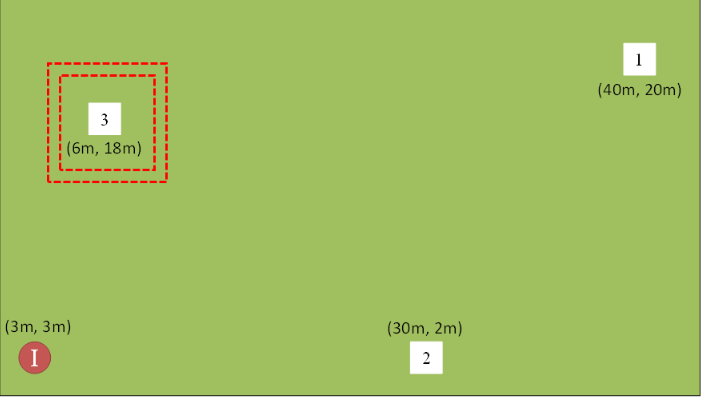
\includegraphics[width=0.8\linewidth]{imgs/trekking_campo.png}
	\caption{Ilustração do ambiente ao qual o robô está inserido}
\end{figure}

\subsection{Um robô para o desafio}
\paragraph{}
O \emph{Projeto Piranha} é um robô desenvolvido pela equipe \tit{Phoenix} de
robótica da Unicamp -- uma equipe de estudantes de graduação da computação e
diversas engenharias -- para executar as tarefas propostas pelo desafio 
\tit{Trekking}. 
A sua estrutura mecânica é um automodelo elétrico projetado para andar a altas
velocidades em terrenos acidentados. Faz-se uso de diversos sensores inerciais,
como magnetômetro, acelerômetro e giroscópio, além de uma câmera USB.
O processamento principal é executado em uma \tit{GPU} embarcada 
\tit{NVIDIA Jetson TX1}.

\begin{figure}[H]
	\centering
	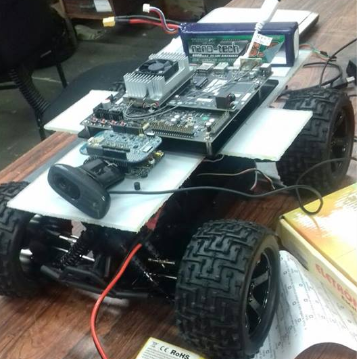
\includegraphics[width=0.6\linewidth]{imgs/piranha.png}
	\caption{O Projeto Piranha e seus componentes}
\end{figure}

A estratégia adotada atualmente divide o problema de se ir de uma base a outra
em duas etapas. 
Na primeira, o robô está relativamente distante da base a se 
chegar (por volta de dez metros). Nessa etapa, faz-se uso de sensores inerciais
e um controle PID para que o robô faça uma trajetória retilínia até os 
arredores da base. 
Na segunda etapa, já a uma distância menor de dez metros, deve-se corrigir o 
erro na direção acumulado pela etapa anterior para que o robô chegue de fato
em cima da base. Para isso, usa-se a câmera embarcada, com técnicas de
visão computacional a serem desenvolvidas neste trabalho.

\subsection{Sistemas robóticos com GPUs embarcadas}
\paragraph{}
Falar o diferencial de GPUs para certos tipos de operações,
como o uso de GPUs em robôs embarcados é recente e o que isso pode trazer de
benefícios (não-limitação).

\subsection{Visão computacional para a solução do problema}
\paragraph{}
A natureza dos desafios torna o uso de visão computacional uma alternativa
considerada a ser usada para solucionar alguns dos principais problemas
da categoria. 
Na etapa com obstáculos, o uso de câmera é novamente uma alternativa para 
que se detecte onde estão os objetos dos quais deve-se desviar.
Com o fato que o sistema é robótico e então deve-se ter uma resposta em uma 
janela de tempo satisfatória, o que se busca são técnicas confiáveis e 
eficientes que permitam ao robô ter, a partir da imagem da câmera, informações
suficientes para que se possa navegar por um ambiente com locais a 
se chegar e obstáculos esparsos.

\subsection{Processos atencionais}
\paragraph{}

\subsection{Aprendizado de máquina aplicado a reconhecimento de padrões}
\paragraph{}

\section{Objetivos}
\paragraph{}
Ao abstrair os problemas específicos da categoria, fica evidente que o que se
busca são técnicas de análise de imagem que permitam, com robustez e eficiência,
identificar e classificar diferentes entidades.
-Falar sobre como se planeja fazer isso mesclando PA e ML.

\section{Métodos}
\paragraph{}
Bla bla bla. 

\section{Cronograma}
\paragraph{}
Bla bla bla.

\section{Referências}
\paragraph{}
Bla bla bla.

\end{document}
